\documentclass{beamer}

\usepackage{polyglossia}

\usepackage[orientation = portrait, size = a0, scale = 1.4]{beamerposter}
\usepackage[backend = biber, style = iso-authoryear, sortlocale = en_US, autolang = other, bibencoding = UTF8]{biblatex}
\usepackage{datetime}
\usepackage[utf8]{inputenc}
\usepackage{fontspec}
\usepackage{microtype}

\setdefaultlanguage{english}
\setmainfont{TeX Gyre Termes}
\usetheme{gemini}
\usecolortheme{mit}

\addbibresource{zotero.bib}
\AtBeginBibliography{\small}

\title{Balancing performance and complexity with adaptive graph coarsening}

\newdate{presentation}{11}{07}{2022}
\date{EEML 2023, \displaydate{presentation}}

\author{Marek Dědič\inst{1, 2}}

\institute{
	\inst{1} Faculty of Nuclear Sciences and Physical Engineering, Czech Technical University in Prague \samelineand
	\inst{2} Cognitive Intelligence, Cisco Systems, Inc.
}


\footercontent{
	EEML 2023, Košice \hfill
	\href{mailto:marek@dedic.eu}{marek@dedic.eu}
}

% \logoright{\includegraphics[height=7cm]{logo1.pdf}}
% \logoleft{\includegraphics[height=7cm]{logo2.pdf}}

% If you have N columns, choose \sepwidth and \colwidth such that
% (N+1)*\sepwidth + N*\colwidth = \paperwidth
\newlength{\sepwidth}
\newlength{\colwidth}
\setlength{\sepwidth}{0.033\paperwidth}
\setlength{\colwidth}{0.45\paperwidth}
\newcommand{\separatorcolumn}{\begin{column}{\sepwidth}\end{column}}

\begin{document}

\begin{frame}[t]

\begin{columns}[t]
	\separatorcolumn

	\begin{column}{\colwidth}
		\begin{block}{Motivation}
			Graph neural networks (GNNs) have proven to achieve superior performance on a number of graph datasets and are adopted in industrial applications across many fields. Superior GNN performance is, however, often paid for by a numerically intensive training procedure with a significant memory footprint, which may be a prohibitive issue in some applications. We investigate the interplay of graph coarsening and the quality of its learned embedding, which in turn entails an interplay between the coarsening and the performance of a downstream task, in our case, node classification.
			\begin{figure}
				\includegraphics[width=0.7\linewidth]{images/coarsening-illustration/coarsening-illustration.pdf}
			\end{figure}
		\end{block}

		\begin{block}{The performance-complexity trade-off}
			The main aim of our work is to explore the performance-complexity characteristics in the context of graph learning, as introduced in \cite{prochazka_downstream_2022}. The result of a repeated application of graph coarsening is a sequence of graphs \( G_0, G_1, G_2, \dots, G_L \), where \( G_0 = G \). Given a model that operates on graphs, a performance metric, and a complexity metric, the sequence \( G_0, G_1, \dots, G_L \) corresponds to points in the performance-complexity plane, where advancing along the sequence generally hurts performance and decreases complexity. This performance-complexity characteristic allows for a choice of a working point that is optimal for the particular use-case.

			\begin{figure}
				\includegraphics[width=0.8\linewidth]{images/performance-complexity/performance-complexity.pdf}
			\end{figure}
		\end{block}

		\begin{block}{HARP pipeline overview}
			Our work builds on the HARP method (see \cite{chen_harp_2018}) for pretraining on coarsened graphs. In HARP, the graph is coarsened using a pre-defined schema and the embedding is trained on the coarser graph first, prolonged to the original graph and finally trained on that as well.
			\begin{figure}
				\includegraphics[width=\linewidth]{images/harp-overview/harp-overview.pdf}
			\end{figure}
		\end{block}
	\end{column}

	\separatorcolumn

	\begin{column}{\colwidth}
		\begin{block}{Deep HARP}
			The one-level HARP schema is generalized to obtain the sequence \( G_0, G_1, G_2, \dots, G_L \) by repeatedly coarsening the graph. Subsequently, the method consists of alternating steps of training the embedding \( \Phi_{G_i} \) on an intermediary graph \( G_i \), followed by a prolongation to \( G_{i - 1} \), going from the coarsest graph \( G_L \) to the original \( G_0 \).
			\begin{figure}
				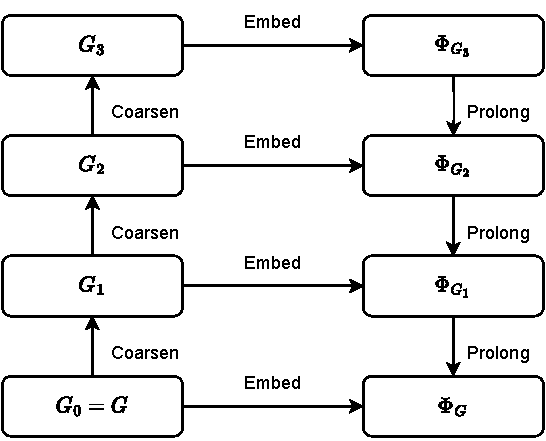
\includegraphics[width=0.5\linewidth]{images/deep-harp/deep-harp.pdf}
			\end{figure}
		\end{block}

		\begin{block}{Adaptive prolongation}

			The main contribution of our work is the introduction of the adaptive prolongation scheme. The algorithm works with the pre-coarsened graphs produced by HARP, however, the prolongation steps are decoupled from the coarsening steps. The prolongation steps are driven by local properties of the graph with relation to the downstream task, allowing for different levels of granularity in different parts of the graph. A single prolongation step is illustrated below.

			\begin{figure}
				\includegraphics[width=\linewidth]{images/adaptive-prolongation/adaptive-prolongation.pdf}
			\end{figure}
		\end{block}

		\begin{block}{Results}
			Downstream classifier accuracies at different steps of adaptive prolongation. Dashed line shows the baseline node2vec model accuracy. The node count is taken relative to the total node count in each dataset. The results are averaged over multiple runs, with the solid line representing the mean and the shaded area denoting one standard deviation.
			\begin{figure}
				\includegraphics[width = \linewidth]{images/adaptive-coarsening/adaptive-coarsening.pdf}
			\end{figure}
		\end{block}

		\begin{block}{References}
			\printbibliography
		\end{block}
	\end{column}

	\separatorcolumn
\end{columns}

\end{frame}

\end{document}
